\mode*

\subsection{Réflexions préliminaires}
\begin{frame}[fragile]{Spécification du problème}

\begin{block}{Interface du verrou}
\begin{lstlisting}[numbers=none]
interface Lock {
  void lock() ;
  void unlock() ;
}
\end{lstlisting}
\end{block}

\begin{block}{Spécification logique}
\begin{description}
\item[Exclusion mutuelle : ] Il ne peut jamais y avoir deux threads en section critique en même temps
\item[Starvation-freedom : ] Si un thread cherche à entrer en section critique, il finira par entrer en section critique
\end{description}
\end{block}
\end{frame}


\begin{frame}[fragile]{Un premier essai}
  \begin{tikzpicture}
    \draw (2,8.5) node{
    \begin{tikzpicture}
    \fill[exampleColor!20, rounded corners] (4.25,5.9) rectangle (8.3,6.2);
    \fill[structure!20, rounded corners] (3.1,4.85) rectangle (5.8,5.55);
    \fill[alertColor!20, rounded corners] (3.1,3.85) rectangle (5.8,4.15);

\draw (5,4.85) node{\begin{minipage}{5cm}\begin{lstlisting}[numbers=none]
class NaiveLock1 implements Lock {
  private boolean taken = false;
  public void lock() {
    while(taken);
    taken = true;
  }
  public void unlock() {
    taken = false;
  }
}
\end{lstlisting}\end{minipage}};
  \end{tikzpicture}};

\uncover<1>{
  \draw (4.5,5) node{\begin{minipage}{\textwidth}
  \begin{exampleblock}{Exercice}

  \vspace{2mm}
   Deux threads veulent entrer concurrament en section critique.

  \vspace{2mm}
  \begin{itemize}
  \item Tracer la machine à états du système. 
  \item Montrer que l'exclusion mutuelle n'est pas respectée
  \item Montrer que la starvation-freedom n'est pas respectée
  \end{itemize}
  \end{exampleblock}
  \end{minipage}};
}

\uncover<2->{
  \draw (5,5) node{\begin{tikzpicture}
  \newcommand\tinylst[1]{\scalebox{.5}{\lstinline{#1}}}

   \draw[exampleColor, fill=exampleColor!10, ultra thin, rounded corners] (0,6)    +(-.5,-.35) rectangle +(1.1,.35);
   \draw[structure]    (0,6.2)  node[left]{\tinylst{taken}} node {\tiny=} node[right]{\tinylst{false}};
   \draw               (0,6)    node[left]{\tiny$t1$} node {\tiny:} node[right]{\tinylst{while(taken)}};
   \draw               (0,5.8)  node[left]{\tiny$t2$} node {\tiny:} node[right]{\tinylst{while(taken)}};

   \draw[fill=black!10, ultra thin, rounded corners] (3,6)    +(-.5,-.35) rectangle +(1.1,.35);
   \draw[structure]    (3,6.2)  node[left]{\tinylst{taken}} node {\tiny=} node[right]{\tinylst{false}};
   \draw               (3,6)    node[left]{\tiny$t1$} node {\tiny:} node[right]{\tinylst{taken = true}};
   \draw               (3,5.8)  node[left]{\tiny$t2$} node {\tiny:} node[right]{\tinylst{while(taken)}};

   \draw[fill=black!10, ultra thin, rounded corners] (6,6)    +(-.5,-.35) rectangle +(1.1,.35);
   \draw[structure]    (6,6.2)  node[left]{\tinylst{taken}} node {\tiny=} node[right]{\tinylst{true}};
   \draw               (6,6)    node[left]{\tiny$t1$} node {\tiny:} node[right]{\tiny SC};
   \draw               (6,5.8)  node[left]{\tiny$t2$} node {\tiny:} node[right]{\tinylst{while(taken)}};


   \draw[fill=black!10, ultra thin, rounded corners] (0,4.7)  +(-.5,-.35) rectangle +(1.1,.35);
   \draw[structure]    (0,4.9)  node[left]{\tinylst{taken}} node {\tiny=} node[right]{\tinylst{false}};
   \draw               (0,4.7)  node[left]{\tiny$t1$} node {\tiny:} node[right]{\tinylst{while(taken)}};
   \draw               (0,4.5)  node[left]{\tiny$t2$} node {\tiny:} node[right]{\tinylst{taken = true}};

   \draw[fill=black!10, ultra thin, rounded corners] (3,4.7)  +(-.5,-.35) rectangle +(1.1,.35);
   \draw[structure]    (3,4.9)  node[left]{\tinylst{taken}} node {\tiny=} node[right]{\tinylst{false}};
   \draw               (3,4.7)  node[left]{\tiny$t1$} node {\tiny:} node[right]{\tinylst{taken = true}};
   \draw               (3,4.5)  node[left]{\tiny$t2$} node {\tiny:} node[right]{\tinylst{taken = true}};

   \draw[fill=black!10, ultra thin, rounded corners] (6,4.7)  +(-.5,-.35) rectangle +(1.1,.35);
   \draw[structure]    (6,4.9)  node[left]{\tinylst{taken}} node {\tiny=} node[right]{\tinylst{true}};
   \draw               (6,4.7)  node[left]{\tiny$t1$} node {\tiny:} node[right]{\tiny SC};
   \draw               (6,4.5)  node[left]{\tiny$t2$} node {\tiny:} node[right]{\tinylst{taken = true}};


   \draw[fill=black!10, ultra thin, rounded corners] (0,3.4)    +(-.5,-.35) rectangle +(1.1,.35);
   \draw[structure]    (0,3.6)  node[left]{\tinylst{taken}} node {\tiny=} node[right]{\tinylst{true}};
   \draw               (0,3.4)    node[left]{\tiny$t1$} node {\tiny:} node[right]{\tinylst{while(taken)}};
   \draw               (0,3.2)  node[left]{\tiny$t2$} node {\tiny:} node[right]{\tiny SC};

   \draw[fill=black!10, ultra thin, rounded corners] (3,3.4)    +(-.5,-.35) rectangle +(1.1,.35);
   \draw[structure]    (3,3.6)  node[left]{\tinylst{taken}} node {\tiny=} node[right]{\tinylst{true}};
   \draw               (3,3.4)    node[left]{\tiny$t1$} node {\tiny:} node[right]{\tinylst{taken = true}};
   \draw               (3,3.2)  node[left]{\tiny$t2$} node {\tiny:} node[right]{\tiny SC};

   \draw<3>[alertColor,fill=alertColor!20, ultra thin, rounded corners] (6,3.4)    +(-.5,-.35) rectangle +(1.1,.35);
   \draw<2,4>[fill=black!10, ultra thin, rounded corners] (6,3.4)    +(-.5,-.35) rectangle +(1.1,.35);
   \draw[structure]    (6,3.6)  node[left]{\tinylst{taken}} node {\tiny=} node[right]{\tinylst{true}};
   \draw               (6,3.4)  node[left]{\tiny$t1$} node {\tiny:} node[right]{\tiny SC};
   \draw               (6,3.2)  node[left]{\tiny$t2$} node {\tiny:} node[right]{\tiny SC};

   \draw[-latex]               (-1,6) -- (-.5,6);

   \draw[structure, -latex]    (0.3,5.65) -- (0.3,5.05);
   \draw[structure, -latex]    (0.3,4.35) -- (0.3,3.75);
   \draw<2,4>[structure, -latex]    (3.3,5.65) -- (3.3,5.05);
   \draw<2,4>[structure, -latex]    (3.3,4.35) -- (3.3,3.75);
   \draw<3>[alertColor, -latex]    (3.3,5.65) -- (3.3,5.05);
   \draw<3>[alertColor, -latex]    (3.3,4.35) -- (3.3,3.75);
   \draw[structure, -latex]    (6.3,4.35) -- (6.3,3.75);
   

   \draw[structure, -latex]    (1.1,4.7) -- (2.5,4.7);
   \draw[structure, -latex]    (4.1,4.7) -- (5.5,4.7);
   \draw<2,4>[structure, -latex]    (4.1,3.4) -- (5.5,3.4);
   \draw<3>[alertColor, -latex]    (4.1,3.4) -- (5.5,3.4);

   \draw[structure, -latex]    (1.1,3.3 ) to[out=-20,in=20,distance=15] (1.1,3.5);

     \draw<-3>[structure, -latex]    (6.2,5.65) to[out=-110,in=-80,distance=15] (6.4,5.65);
     \draw<2>[structure, -latex]    (1.1,6.0) -- (2.5,6.0);
     \draw<-3>[structure, -latex]    (4.1,6.0) -- (5.5,6.0);
     \draw<3->[alertColor, -latex]    (1.1,6.0) -- (2.5,6.0);
     \draw<4>[alertColor, -latex]    (4.1,6.0) -- (5.5,6.0);
     \draw<4>[alertColor, -latex]    (6.2,5.65) to[out=-110,in=-80,distance=15] (6.4,5.65);

     \uncover<4>{
       \draw[alertColor, -latex, rounded corners]    (6.3,6.35) -- (6.3,6.6) -- (0.3,6.6) -- (0.3,6.35);
     }

\end{tikzpicture}};
   }
 \end{tikzpicture}
\end{frame}


\begin{frame}[fragile]{Un deuxième essai}

On suppose deux processus, d'identifiants 0 et 1. 

    \begin{tikzpicture}
    \fill[structure!20, rounded corners] (4.25,6.2) rectangle (13.5,6.5);
    \fill[structure!20, rounded corners] (3.1,4.85) rectangle (7.5,5.55);
    \fill[structure!20, rounded corners] (3.1,3.55) rectangle (7.2,3.85);

\draw (5,4.85) node{\begin{minipage}{5cm}\begin{lstlisting}[numbers=none]
class NaiveLock2 implements Lock {
  private boolean[] entering = new boolean[]{false, false};
  public void lock() {
    int i = ThreadID.get();
    entering[i] = true; 
    while(entering[1-i]);
  }
  public void unlock() {
    int i = ThreadID.get();
    entering[i] = false;
  }
}
\end{lstlisting}\end{minipage}};
  \end{tikzpicture}

  \begin{exampleblock}{Exercice}

  \vspace{2mm}
  \begin{itemize}
  \item Cet algorithme respecte-t-il l'exclusion mutuelle ?
  \item Cet algorithme est-il starvation-free ?
  \end{itemize}
  \end{exampleblock}

\end{frame}


\begin{frame}[fragile]{Un troisième essai}

On suppose deux processus, d'identifiants 0 et 1. 

\begin{tikzpicture}
    \fill[exampleColor!20, rounded corners] (4.25,5.9) rectangle (7.4,6.2);
    \fill[exampleColor!20, rounded corners] (3.1,4.85) rectangle (7.1,5.2);
    \fill[exampleColor!20, rounded corners] (3.1,3.55) rectangle (6.0,3.85);

\draw (5,4.7) node{\begin{minipage}{5cm}\begin{lstlisting}[numbers=none]
class NaiveLock3 implements Lock {
  private int priority = 0;
  public void lock() {
    int i = ThreadID.get();
    while(priority != i);
  }
  public void unlock() {
    int i = ThreadID.get();
    priority = 1-i;
  }
}
\end{lstlisting}\end{minipage}};
  \end{tikzpicture}

  \begin{exampleblock}{Exercice}

  \vspace{2mm}
  \begin{itemize}
  \item Cet algorithme respecte-t-il l'exclusion mutuelle ?
  \item Cet algorithme est-il starvation-free ?
  \end{itemize}
  \end{exampleblock}
\end{frame}

\subsection{Algorithme de Peterson}

\begin{frame}[fragile]{Algorithme de Peterson}
On suppose deux processus, d'identifiants 0 et 1. 

\begin{tikzpicture}
    \fill[exampleColor!20, rounded corners] (4.25,5.85) rectangle (7.4,6.15);
    \fill[exampleColor!20, rounded corners] (3.1,4.55) rectangle (6.0,4.82);
    \fill[structure!20, rounded corners] (4.25,6.2) rectangle (13.2,6.5);
    \fill[structure!20, rounded corners] (3.1,4.835) rectangle (7.0,5.15);
    \fill[structure!20, rounded corners] (3.1,2.85) rectangle (7.0,3.15);

\draw (5,4.5) node{\begin{minipage}{5cm}\begin{lstlisting}[numbers=none]
class PetersonLock implements Lock {
  private boolean[] entering = new boolean[]{false, false};
  private int priority = 0;
  public void lock() {
    int i = ThreadID.get();
    entering[i] = true;
    priority = 1-i;
    while(entering[1-i] && priority != i);
  }
  public void unlock() {
    int i = ThreadID.get();
    entering[i] = false;
  }
}
\end{lstlisting}\end{minipage}};
  \end{tikzpicture}

\vspace{-3mm}
  \begin{exampleblock}{Exercice}
  \begin{itemize}
  \item Cet algorithme respecte-t-il l'exclusion mutuelle ?
  \item Cet algorithme est-il starvation-free ?
  \end{itemize}
  \end{exampleblock}

  \vspace{-1mm}
  \begin{citing}
  \item Gary L. Peterson. \textit{Myths About the Mutual Exclusion Problem.} IPL (1981)
  \jitem \lstinline{cm5/PetersonLock.java}
  \end{citing}
\end{frame}



\subsection{Algorithme de la Boulangerie de Lamport}

\begin{frame}[fragile]{Algorithme simplifié}

  \scalebox{.9}{
    \begin{tikzpicture}

      \draw (10.8,0) node{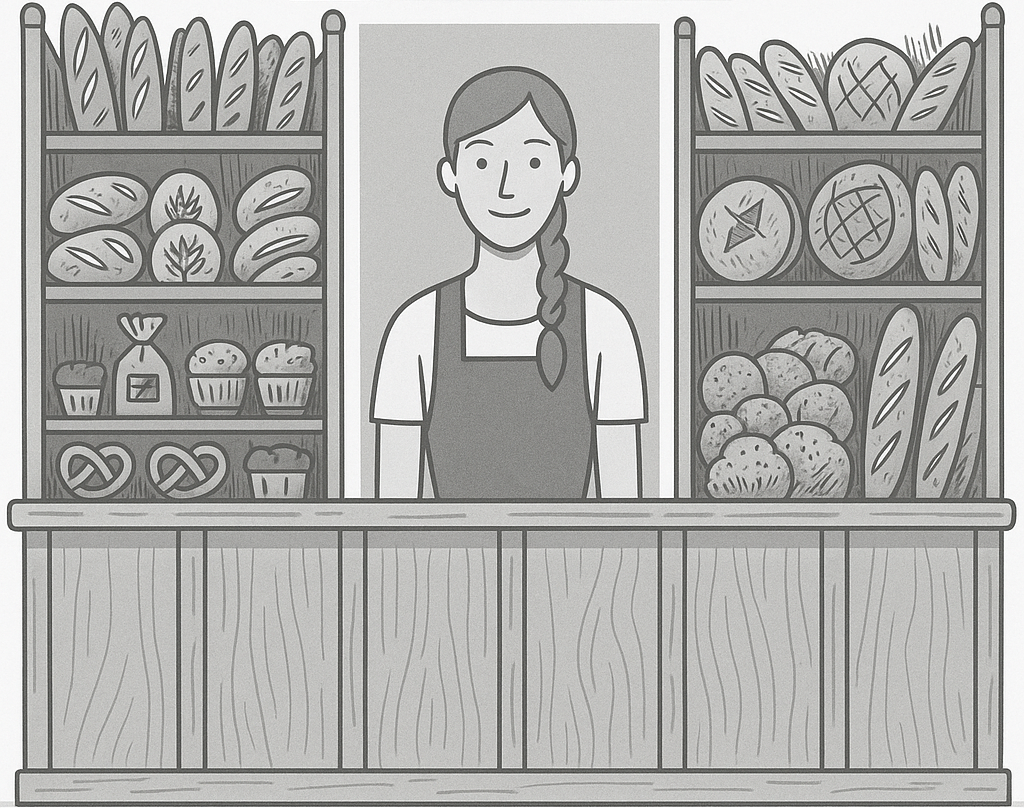
\includegraphics[height=3.3cm]{bakery}};

    \fill<2>[rounded corners, structure!20]       (0,6.6) rectangle (3.8,7.05);
    \fill<2>[rounded corners, structure!20]       (0,2.65) rectangle (2.55,3.1);

    \fill<3>[rounded corners, structure!20] (0,5.5)  rectangle (2.4,5.95);
    \fill<4>[rounded corners, structure!20] (0,4.35) rectangle (7.3,5.5);
    \fill<5>[rounded corners, structure!20] (0,3.7)  rectangle (5.5,4.4);
    
    \draw<2>   (10.8,5) node{
\includegraphics[height=2.5cm]{frenchieBleu}};
    \draw<4>   (1,0)    node{
\includegraphics[height=2.5cm]{frenchieDroit}};
    \draw<2-4> (3.2,0)  node{
\includegraphics[height=2.5cm]{frenchieRouge}};
    \draw<2-4> (5.4,0)  node{
\includegraphics[height=2.5cm]{frenchieVert}};
    \draw<3>   (7.6,0)  node{
\includegraphics[height=2.5cm]{frenchieBleu}};
    \draw<5>   (7.5,0)  node{
\includegraphics[height=2.5cm]{frenchieDroit}};

    \draw<2>  [structure]    (10.7,4.7) node{\Large $\infty$};
    \draw<4>  [structure]    (1.1,-.3)  node{\Large $3$};
    \draw<2-4>[alertColor]   (3.3,-.3)  node{\Large $2$};
    \draw<2-4>[exampleColor] (5.5,-.3)  node{\Large $1$};
    \draw<3>  [structure]    (7.5,-.3)  node{\Large $0$};
    \draw<5>  [structure]    (7.6,-.3)  node{\Large $3$};

    \draw<6> (4,1.4) node{\begin{minipage}{.8\textwidth}
        \begin{block}{Exclusion mutuelle:}
          \vspace{-3mm}
          Supposons $p_i$ et $p_j$ en section critique, avec $\left\langle t_i,i \right\rangle < \left\langle t_j,j \right\rangle$
        \end{block}
    \end{minipage}};

    \draw<6>[->] (0.25,0) node[left]{$p_i$} -- (6.8,0) ;
    \draw<6>[->] (0.25,-.75 ) node[left]{$p_j$} -- (6.8,-.75) ;
    
    \draw<6>[rounded corners, exampleColor, fill=exampleColor!20] (1.75,0)    node{\scriptsize 1: $tickets[i] \leftarrow 0$}   +(-1.3,-.25) rectangle +(1.3,.25);
    \draw<6>[rounded corners, alertColor,   fill=alertColor!20]   (4.9,0)     node{\scriptsize 2: $tickets[j] \rightarrow {<t_j} $}    +(-1.6,-.25) rectangle +(1.6,.25);
    \draw<6>[rounded corners, alertColor,   fill=alertColor!20]   (1.75,-.75) node{\scriptsize 3: $tickets[j] \leftarrow t_j$} +(-1.3,-.25) rectangle +(1.3,.25);
    \draw<6>[rounded corners, exampleColor, fill=exampleColor!20] (4.9,-.75)  node{\scriptsize 4: $tickets[i] \rightarrow \infty$}    +(-1.6,-.25) rectangle +(1.6,.25);
    
    \fill<6>[rounded corners, exampleColor!20] (0,5.5)    rectangle (2.5,5.95);
    \fill<6>[rounded corners, alertColor!20]   (5.2,5.05)  rectangle (7.2,5.5);
    \fill<6>[rounded corners, alertColor!20]   (0,4.35)   rectangle (2.5,4.8);
    \fill<6>[rounded corners, exampleColor!20] (3.45,3.9) rectangle (5.45,4.4);
    
    \draw (5,5) node{\begin{minipage}{\textwidth}
        \begin{algorithm}[H]
        \SetKwFunction{Lock}{lock}
        \SetKwFunction{Unlock}{unlock}
          \SubAlgo{\structure{\textbf{shared variables}}}{
            $tickets[n] \leftarrow [\infty, ..., \infty]$\;
          }
          ~\\
          \SubAlgo{\structure{\textbf{operation}} $\Lock()$}{
            \nl $tickets[i] \leftarrow 0$\;
            \nl \structure{\textbf{let}} $t_i$ \structure{\bf such that} $\displaystyle \left\langle t_i,i \right\rangle > \max_{j : tickets[j] < \infty} \left\langle tickets[j], j\right\rangle$\;
            \nl $tickets[i] \leftarrow t_i$\;
            \nl \structure{\textbf{wait until}} $\displaystyle \left\langle t_i,i \right\rangle = \min_j \left\langle tickets[j], j \right\rangle$.
          }
          ~\\
          \SubAlgo{\structure{\textbf{operation}} $\Unlock()$}{
            $tickets[i] \leftarrow \infty$.
          }
        \end{algorithm}
    \end{minipage}};

    \end{tikzpicture}
    
  }
\end{frame}




\begin{frame}[fragile]{Algorithme de Lamport}
\begin{tikzpicture}
    \fill[exampleColor!20, rounded corners] (4.25,5.85) rectangle (8.8,6.15);
    \fill[exampleColor!20, rounded corners] (3.2,4.65) rectangle (8.5,4.95);
    \fill[exampleColor!20, rounded corners] (3.2,2.25) rectangle (6,2.55);
    \fill[exampleColor!20, rounded corners] (3.2,0.45) rectangle (10.2,1.65);
    \fill[exampleColor!20, rounded corners] (6.9,3.75) rectangle (10.5,4.05);
    \fill[structure!20, rounded corners] (4.25,6.2) rectangle (10.2,6.5);
    \fill[structure!20, rounded corners] (3.2,4.95) rectangle (6.5,5.25);
    \fill[structure!20, rounded corners] (3.2,4.35) rectangle (6.5,4.65);
    \fill[structure!20, rounded corners] (4.55,3.75) rectangle (6.5,4.05);

\draw (8,3.3) node[scale=.9]{\begin{minipage}{1.1\textwidth}\begin{lstlisting}[numbers=none]
class BakeryLock implements Lock {
  private boolean[] entering = new boolean[n]; // {false...}
  private int[] priority = new int[n]; // {0...}
  public void lock() {
    int i = ThreadID.get();
    entering[i] = true;
    priority[i] = 1 + max(priority);
    entering[i] = false;
    for(int j = 0; j < n; j++) {
      while(entering[j] || hasPriorityOverI(j));
    }
  }
  public void unlock() {
    int i = ThreadID.get();
    priority[i] = 0;
  }
  private boolean hasPriorityOverI(int j) {
    if(priority[j] == 0) return false;
    if(priority[j] < priority[i]) return true;
    if(priority[j] == priority[i]) return j<i;
    return false;
  }
}
\end{lstlisting}\end{minipage}};
  \end{tikzpicture}

  \vspace{-2mm}
  \begin{citing}
  \item[L74] Leslie Lamport. \textit{A new solution of Dijkstra's concurrent programming problem.} CACM (1974)
  \jitem \lstinline{cm5/BakeryLock.java}
  \end{citing}

\end{frame}

\subsection{Algorithme spin-lock}

\begin{frame}[fragile]{L'algorithme spin-lock}

\begin{tikzpicture}
    \fill[structure!20, rounded corners] (4.25,5.7) rectangle (12.8,6.0);
    \fill[structure!20, rounded corners] (4.25,4.7) rectangle (8.1,5.0);
    \fill[structure!20, rounded corners] (3.1,3.35) rectangle (6.4,3.65);

\draw (5,4.5) node{\begin{minipage}{5cm}\begin{lstlisting}[numbers=none]
class SpinLock {
  private AtomicBoolean taken = new AtomicBoolean(false);

  public void lock() {
    while(taken.getAndSet(true));
  }

  public void unlock() {
    taken.set(false);
  }
}
\end{lstlisting}\end{minipage}};
  \end{tikzpicture}

\begin{block}{L'opération \alert{atomique} test-and-set}
    \vspace{-2mm}
    \begin{minipage}{.3\textwidth}
    \begin{lstlisting}[numbers=none]
getAndSet(T val) {
  T old = get();
  set(val);
  return old;
}
    \end{lstlisting}
    \end{minipage}
    \hfill    
    \begin{minipage}{.5\textwidth}
    \begin{description}
    \item [Java :] \lstinline{T getAndSet(T val)}
    \item [C++ :] \lstinline{T exchange(T val)}
    \end{description}
    \end{minipage}
    \vspace{-2mm}
  \end{block}

  \vFill
  \begin{citing}
  \item[D62] Edsger W. Dijkstra. \textit{Over de sequentialiteit van procesbeschrijvingen (About the sequentiality of process descriptions)} (1962-1963)
  \jitem \lstinline{cm5/SpinLock.java}
  \end{citing}
\end{frame}


\mode<all>


